% !TeX root = ../../main.tex
% Add the above to each chapter to make compiling the PDF easier in some editors.

\begin{figure}
	\centering
	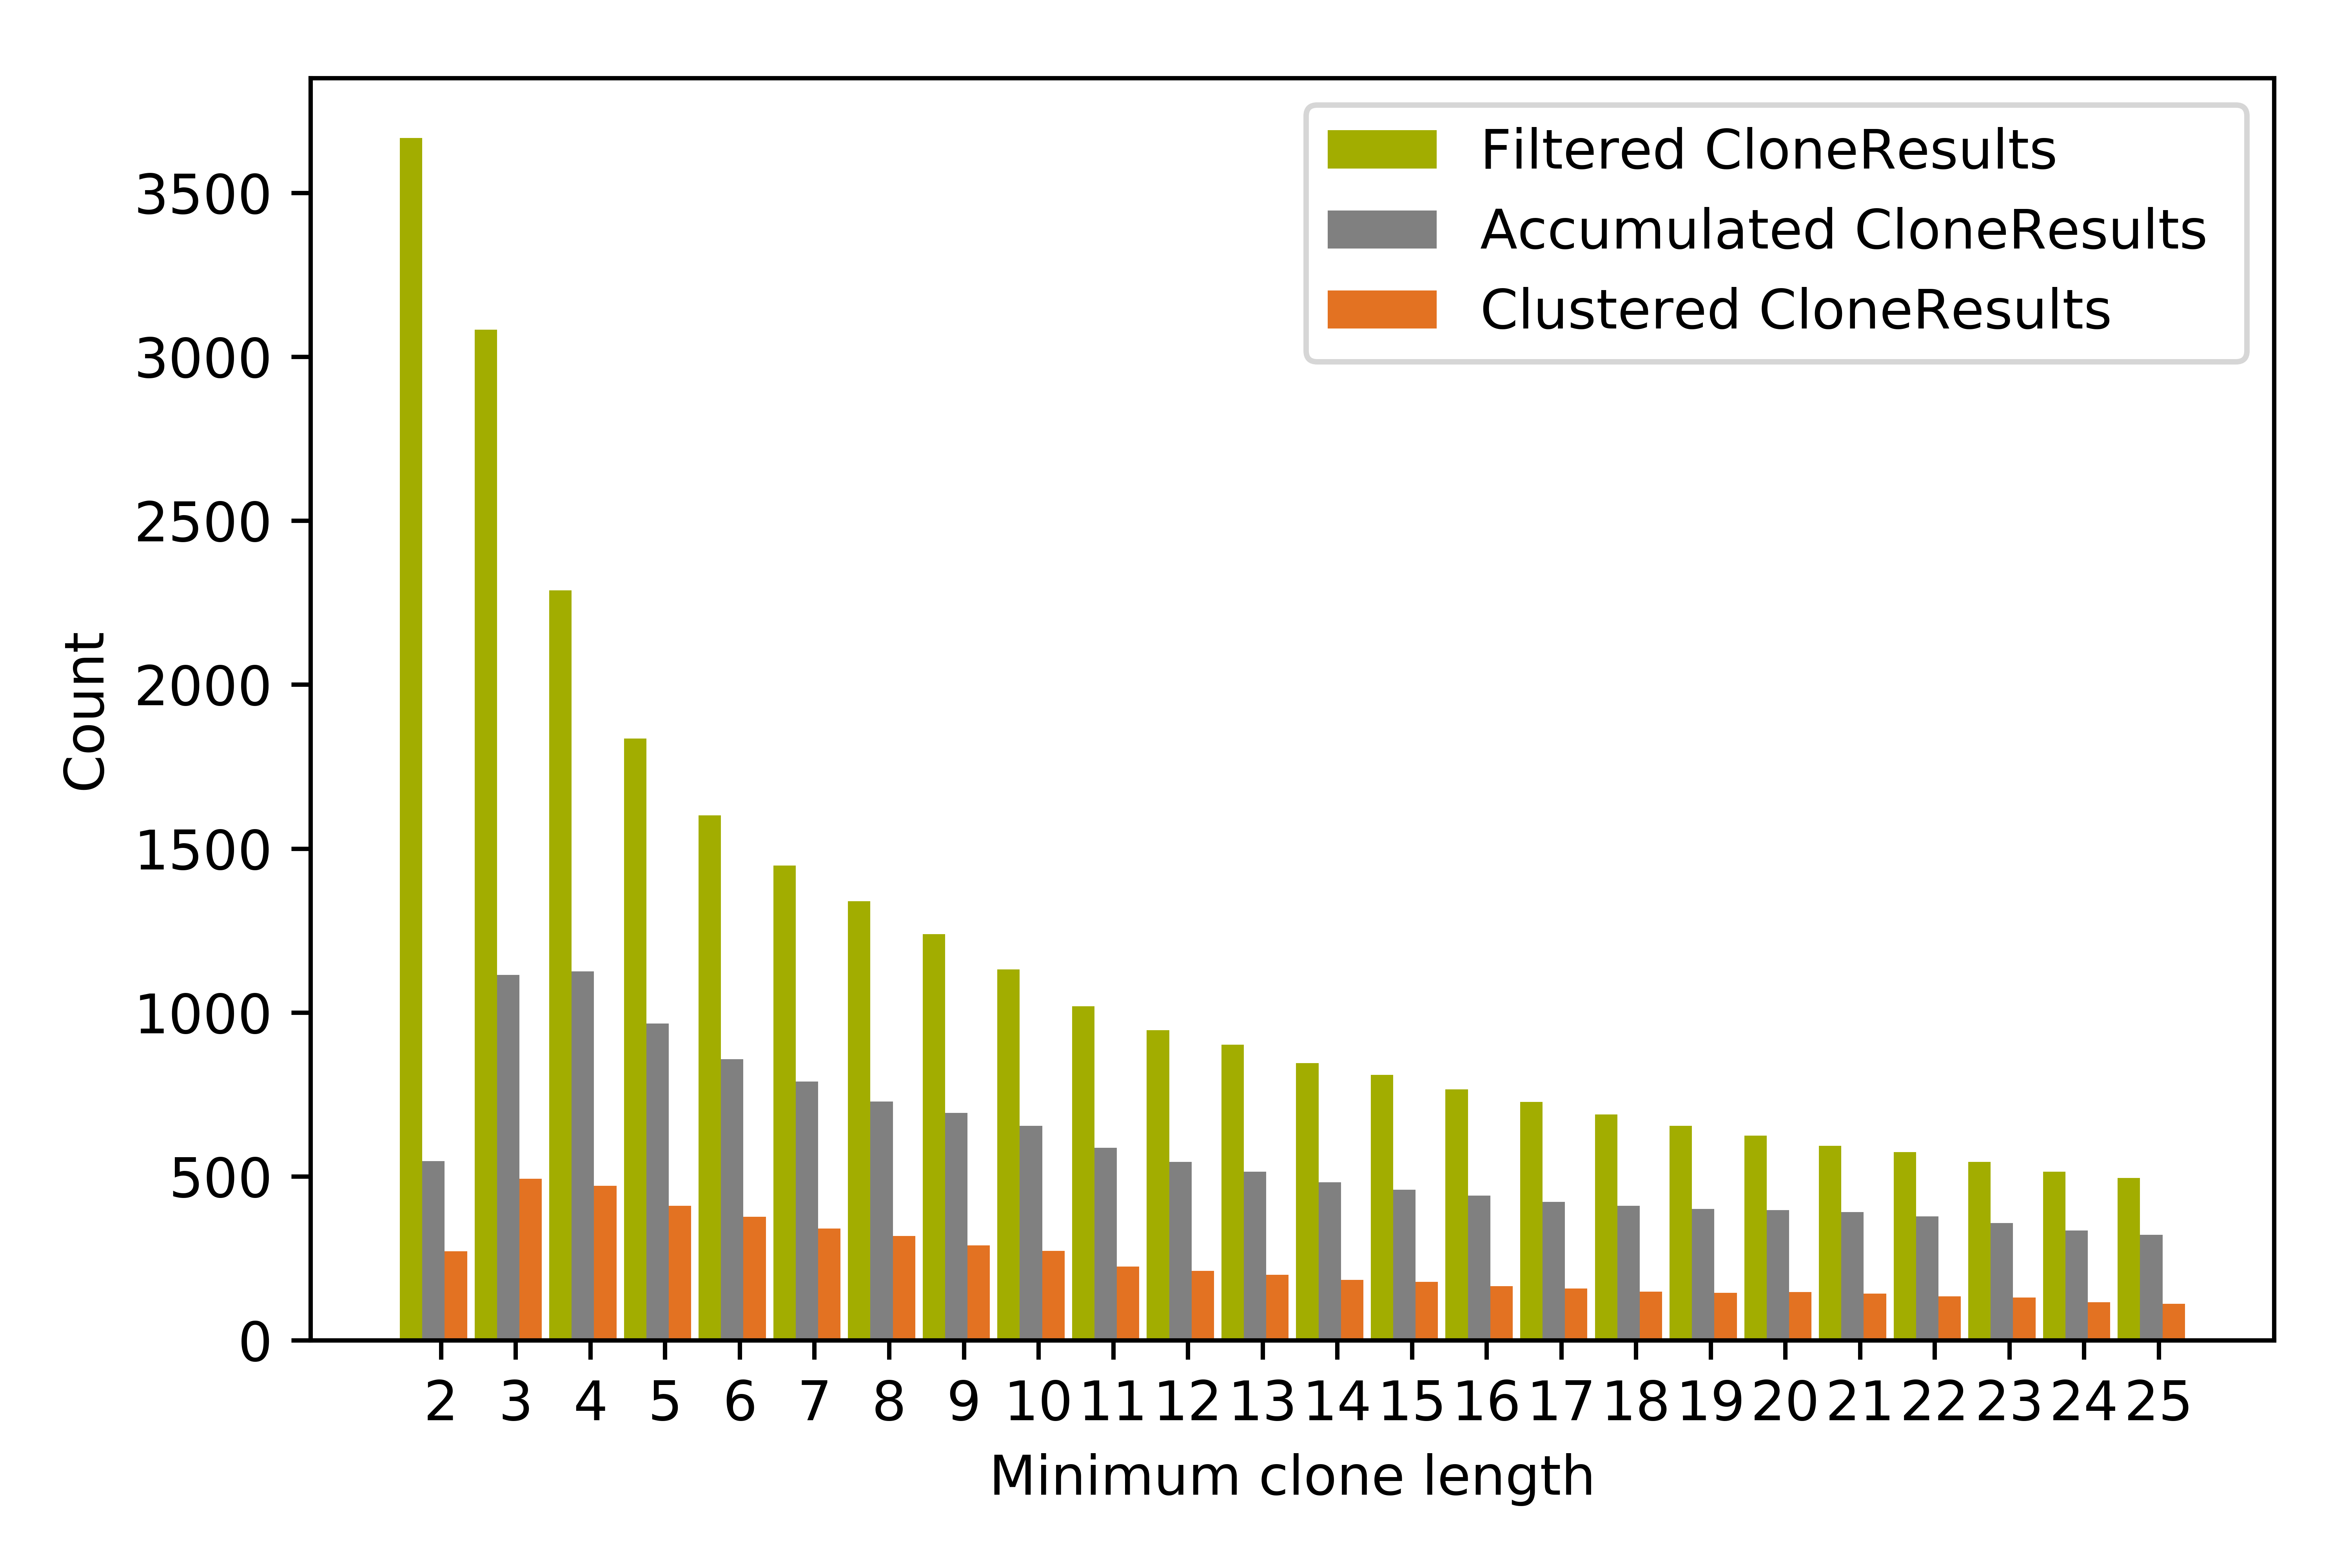
\includegraphics[width=0.8\linewidth]{figures/Thresholds/processed.png}
	\caption[Processed CloneResults in relation to the minimum clone length]{
		The number of
		 \code{CloneResult}s
		  that are left after the three processing steps described in
		   Step~\ref{section:processCloneResults}
		   . The counts are associated to their respective minimum clone length used to find the 
		   \code{CloneResult}s.
	}
	\label{fig:thresholdsProcessed}
\end{figure}
